% this file is called up by thesis.tex
% content in this file will be fed into the main document
\ifpdf
    \graphicspath{{3/figures/PNG/}{3/figures/PDF/}{3/figures/}}
\else
    \graphicspath{{3/figures/EPS/}{3/figures/}}
\fi
\chapter{Technologie} % top level followed by section, subsection


% ----------------------- contents from here ------------------------
W rozdziale tym, zostaną zaprezentowane oraz po krotce opisane najważniejsze technologie wykorzystane przy implementacji systemu SpeechProcessingPlatform. Rysunek \ref{fig:architecture_and_technologies} przedstawia w której części systemu wykorzystywane są poszczególne technologie.

\begin{figure}[!h]
	\centering
	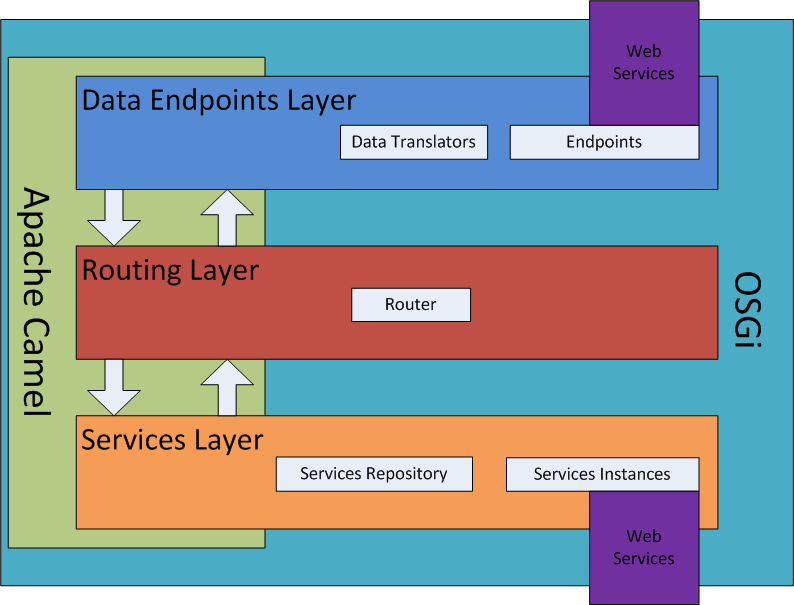
\includegraphics[scale=0.45]{layered_architecture_and_technologies.png} 
	\caption{Architektura systemu SpeechProcessingPlatform wraz z wykorzystywanymi technologiami.}
\label{fig:architecture_and_technologies}
\end{figure}

\section{Technologie integracyjne}
\subsection{OSGi}
Technologia OSGi to zbiór specyfikacji definiujących dynamiczne środowisko komponentowe. Taka struktura pozwala na tworzenie aplikacji złożonych z wielu, różnych komponentów(paczek) które mogą być wykorzystywane wiele razy. Specyfikacja OSGi pozwala komponentowi na ukrywanie swojej implementacji przed innymi i komunikację tylko przy użyciu specjalnych usług, które są dzielone pomiędzy wszystkimi komponentami. Pozwala to na zmniejszenie złożoności tworzonych systemów.

OSGi posiada architekturę warstwową, przedstawiona jest ona, wraz z krótkim opisem, na poniższym diagramie.
\begin{figure}[!h]
	\centering
	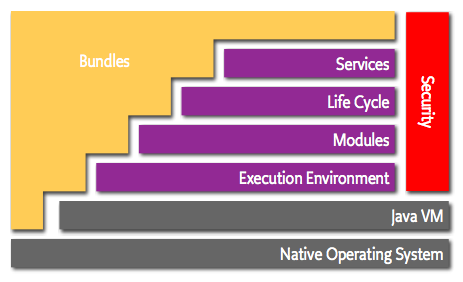
\includegraphics[scale=0.65]{osgiArchitektura.png} 
	\cite{fusehomepage2012}
	\caption{Architektura OSGi}
\end{figure}
\begin{itemize}
	\item Bundles - Są to paczki technologii OSGi, mogą być preinstalowane jak i tworzone i dynamicznie ładowane przez programistów
	\item Services - Warstwa usług dynamicznie łączy komponenty, stosując model publish-find-bin
	\item Life-Cycle - API do startowania, zatrzymywania, instalowania i usuwania komponentów
	\item Modules - Warstwa definiująca jak komponenty mogą importować i eksportować kod	
	\item Security - Warstwa zajmująca się bezpieczeństwem
	\item Execution Environment - Warstwa definiująca jakie metody i klasy są dostępne na specyficznej plarformie
\end{itemize}  
Najważniejszą ideą umożliwiającą istnienie i działanie takiej platformy jest modułowość, której ucieleśnieniem są paczki. OSGi ukrywa wszystko co znajduje się w takim komponencie poza funkcjonalnością która jest wyspecyfikowana. Jeżeli jeden komponent chce wykorzystać inny musi wyraźnie definiować jaką funkcjonalność potrzebuje. Ponieważ ciężko stworzyć model współpracy opierając się tylko na klasach, OSGi wprowadza warstwę usług, a wraz z nią rejestr konkretnych usług. Paczka może stworzyć obiekt i zarejestrować go w rejestrze pod jednym lub więcej interfejsów. Inne komponenty mogą z takiego rejestru pobierać obiekty stosując różne kryteria, na przykład wszystkie obiekty implementujące dany interfejs itd.
\begin{figure}[!h]
	\centering
	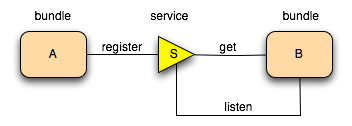
\includegraphics[scale=0.75]{serveLayer.png} 
	\caption{Zależność pomiędzy bundlami i usługami}
\end{figure}
 Możliwe jest oczywiście, żeby dowolna liczba komponentów zarejestrowała ten sam typ usługi lub też pobrała tą samą implementację usługi. Oczywiście zarejestrowane usługi można rozróżniać, każda ma powiązany ze sobą zestaw właściwości(properties), które mogą służyć do specyfikacji. Cała warstwa usług jest dynamiczna, paczki mogą dodawać, usuwać itd. usługi bez konieczności restartu kontenera.  \\
Do tworzenia i definiowana zależności między bundlami OSGi wykorzystuje Blueprint Container. Jest to framework którego celem jest zarządzanie wstrzykiwaniem zależności. Został zaprojektowany żeby radzić sobie z dynamiczną specyfikacją technologii OSGi (możliwość pojawienia się i zniknięcia usługi w dowolnym momencie). Jego specyfikacja pozwala mu też na działania w środowisku innym niż technologii OSGi. W założeniu opiera się on o strukturę plików xml, które definiują jak komponenty są tworzone oraz łączone aby stworzyć działającą aplikację. Sposób działania kontera opiera się o wzorzec Extender. W czasie inicjalizacji paczki (a więc w czasie działania kontenera) Blueprint Container sprawdza czy wszystkie wymagane zależności są spełnione, tworzy wszystkie wymagane obiekty oraz rejestruje usługi. 

Technologia OSGi jest środowiskiem w którym działa budowany system. Każdy komponent systemu jest dostarczany jako osobna paczka OSGi, dzięki czemu może być niezależnie uruchamiany i zarządzany. 

\subsection{Technologia web services}
Technologia web services to system zaprojektowany do wspierania komunikacji między rożnymi komputerami za pomocą sieci.  Podstawowe cechy każdej implementacji tej technologii to:
\begin{itemize}
	\item jest komponentem mogącym być osadzonym w innej aplikacji
	\item komunikacja przy użyciu otwartych protokołów
	\item jest samodzielny i samo-opisujący się
	\item może być zlokalizowany za pomocą UDDI
	\item jest wykorzystywany przez inne aplikacje
\end{itemize}  

Technologia web services jest używana w celu udostępnienia tworzonego systemu jako usługi(Data Endpoints Layer) oraz w celu integracji usług przetwarzania mowy wykorzystujących tą technologię(Services Layer).

Można rozróżnić 2 główne klasy technologii web services :
\begin{itemize}
	\item technologie web services zgodne z architekturą technologii REST
	\item technologie arbitrary web services z których każda może udostępniać dowolny zbiór operacji
\end{itemize}  
\subsubsection{Technologia REST web services}
Usługi z tej grupy \cite{fielding2000} ograniczają swój interfejs do zbioru dobrze znanych i wspieranych przez protokół transportowy operacji takich jak: PUT, GET, POST itd. dla  HTTP. Nacisk jest tutaj skierowany na interakcję z zasobami bezstanowymi. Koncepcja usług technologii REST opiera się na sześciu kluczowych punktach:
\begin{itemize}
	\item model klient-serwer - wprowadza rozdzielenie odpowiedzialności, oznacza to, że na przykład klient nie interesuje się przechowywaniem danych, jest to sprawa wewnętrznej implementacji serwera, a serwer nie interesuje się interfejsem użytkownika co wprowadza prostotę i zwiększa skalowalność
	\item bezstanowość - kontekst aplikacji klienckiej nie jest przechowywany na serwerze pomiędzy zapytaniami, każde nowe zapytanie zawiera wszystkie potrzebne informacje żeby mogło zostać obsłużone
	\item możliwość przechowywania w pamięci podręcznej - aplikacje klienckie mogą przechowywać odpowiedzi w pamięci podręcznej, wymaga to od serwera by odpowiedź była pośrednio lub bezpośrednio zdefiniowana jako możliwa do przechowywania w pamięci podręcznej lub nie, poprawne zarządzanie tą cechą może w sposób znaczny ograniczyć komunikację na linii klient-serwer
	\item warstwowy system - klient nie jest w stanie stwierdzić czy jest bezpośrednio podpięty do usługi czy po drodze znajdują sie inne usługi, takie jak na przykład load-balancer
	\item opcjonalnie wykonanie kodu na żądanie - możliwe jest żeby serwer wykonał kod przesłany przez klienta
	\item jednolity interfejs - upraszcza oraz rozluźnia powiązanie między klientem a serwerem, dzięki temu możliwa jest ich niezależna ewolucja
\end{itemize}   
\subsubsection{Technologia arbitrary web services}
Usługi z tej grupy reprezentują bardziej klasyczne podejście. Do opisania swoich interfejsów mogą (nie jest to wymagane jednak bardzo popularne, co więcej konieczne jeżeli chce się użyć frameworku do generowania kodu) wykorzystywać WSDL. Jest to skrót od Web Service Description Language, formacie bazującym na XML, wykorzystywanym do opisywania jak wywołać daną usługę, jakie parametry wejściowe przyjmuje i jakie struktury danych zwraca. Inne systemy mogą komunikować się z technologią web serwices za pomocą protokołu SOAP. Skrót pochodzi od angielskiej nazwy Simple Object Access Protocol. Dostarcza on standardowy, rozszerzalny, dobrze zdefiniowany fremwork do wymiany wiadomości XML. Wspiera kilka różnych protokołów transportowych takich jak:
 \begin{itemize}
	\item HTTP
	\item SMTP
	\item FTP
	\item RMI/IIOP
\end{itemize}  
\begin{figure}[!h]
	\centering
	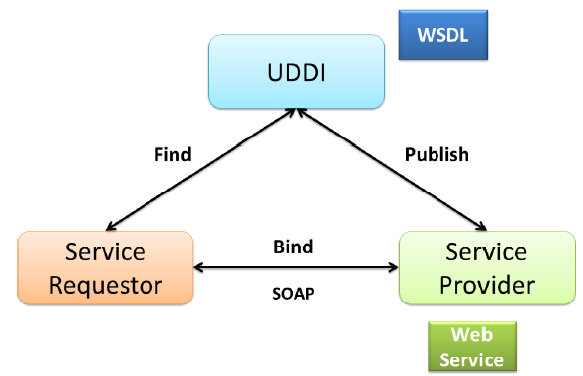
\includegraphics[scale=0.50]{webSerwisyArchitektura.png} 
	\caption{Architektura technologii arbitrary web services}
\end{figure}

\subsection{Apache ServiceMix}
Apache ServiceMix pomaga rozwiązać problem integracji będąc bazującym na standardach, lekkim oraz stosującym paradygmat "luźnego powiązania" narzędziem. Dzięki bazowaniu na standardach w sposób znaczący zmniejsza szanse na uzależnienie się od konkretnego dostawcy oprogramowania, przez stosowanie luźnego powiązania pomiędzy poszczególnymi komponentami zmniejsza złożoność integracji. Jest to otwarta implementacja ESB, zbudowana w oparciu o JBI i wydana na licencji Apache, od wersji 4 ServiceMix wykorzystuje OSGi do uproszczenia podziału aplikacji na komponenty. 	
Architekturę Apache ServiceMix można podzielić na 3 warstwy:
\begin{enumerate}
	\item Warstwa jądra
	\item Warstwa usług
	\item Warstwa aplikacji
\end{enumerate}  
\begin{figure}[!h]
	\centering
	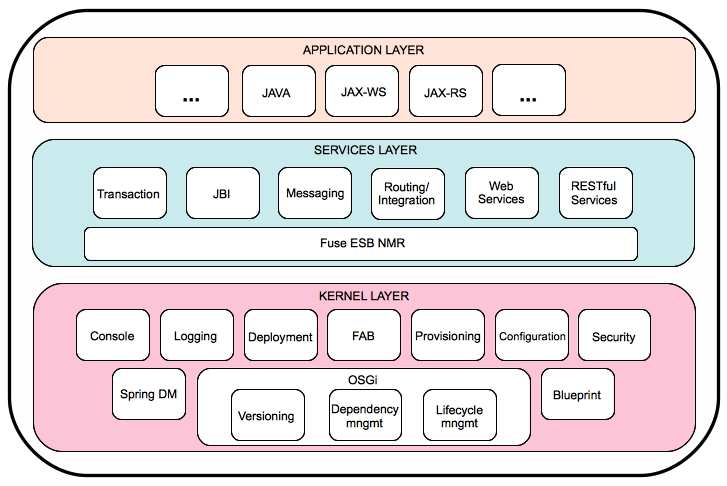
\includegraphics[scale=0.45]{ServiceMixArchitektura.jpg} 
	\caption{Architektura ServiceMix 4}
\end{figure}
Każda z tych warstw ma inne zadania i odpowiada za inne czynności.
\begin{itemize}
	\item Warstwa jądra - bazuje na Apache Karaf czyli implementacji OSGi będącą lekkim kontenerem w którym można osadzić różne komponenty i aplikacje. Warstwa ta współpracuje z warstwą usług w celu stworzenia, skoordynowania, utrzymania i zarządzania logowaniem, bezpieczeństwem oraz transakcjami. Najważniejsze funkcje dostarczane przez tą warstwę to:
	\begin{itemize}
		\item Osadzanie - umożliwia zarówno manualne jak i automatyczne osadzanie bibliotek
		\item Kontener OSGi - ServiceMix 4 wspiera 2 różne kontenery OSGi a mianowicie Eclipse Equinox i Apache Felix
		\item Wstrzykiwanie zależnośći - wykorzystuje 2 różne frameworki:
			\begin{itemize}
				\item Blueprint
				\item Spring DI
			\end{itemize}   
		\item Automatyczna konfiguracja - dokonując zmian w pliku z właściwościami można dokonać zmian "w locie", bez restartowania serwera
		\item Bezpieczeństwo - framework odpowiadający za bezpieczeństwo bazuje na JAAS, dostarcza kilka różnych, odizolowanych poziomów:
			\begin{itemize}
				\item kontenera OSGi
				\item wbudowanej instancji usługi wiadomości
				\item osadzonych instancji usług routingu i integracji
			\end{itemize} 
		\item Logowanie - dynamiczne logowanie wspierające różne interfejsy takie jak: JCL, SLF4J, Avalon, łatwo konfigurowalne poprzez pliki z właściwościami
		\item Konsola - umożliwia zarządzanie i pełną kontrolę nad cała aplikacją
	\end{itemize}  
	\item Warstwa usług - 	składa się z interfejsów i klas reprezentujących wbudowane usługi. Współpracuje z warstwą aplikacji w celu komunikacji z aplikacjami użytkowników które chcą korzystać z oferowanych usług. Najważniejsze funkcje dostarczane przez tą warstwę to:
	\begin{itemize}
		\item Rutowanie i integracja - bazuje na Apache Camel, umożliwia zdefiniowanie ścieżek i zaimplementowanie biznesowych wzorców w celach integracji a następnie osadzenie jako paczka OSGi
		\item Tworzenie usług webowych - bazuje na Apache CXF, umożliwia, w prosty sposób, tworzenie i osadzanie jako paczka OSGi usług webowych implementujących API JAX-WS 
		\item Tworzenie usług webowych zgodnych ze wzorcem REST - bazuje na Apache CXF, umożliwia w prosty sposób, tworzenie i osadzanie jako paczka OSGi usług zgodnych z REST implementujących API JAX-RS
		\item Tworzenie i osadzanie jednostek i zespołów usług bazujących na JBI
		\item Komunikacje - udostępnia usługę wiadomości w całości zbudowaną na Apache ActiveMQ, umożliwiający tworzenie i osadzanie zarówno klientów jak i nadawców wiadomości JMS
		\item Menadżer transakcji - bazuje na Apache Aries, wystawia interfejs transakcji jako usługę, umożliwia tworzenie i osadzanie zarówno aplikacji bazujących na frameworku JTA jak i na technologii Spring
		\item Znormalizowany ruter wiadomości - jego główną rolą jest przekazywanie wiadomości pomiędzy różnymi aplikacjami osadzonymi w kontenerze OSGi oraz, jeżeli zachodzi taka konieczność, pomiędzy aplikacjami z OSGi a aplikacjami osadzonymi w kontenerze JBI
	\end{itemize}
	\item Warstwa aplikacji - w tym miejscu znajdując się aplikacje użytkownika, ServiceMix 4 dostarcza wielu różnych API(częściowo wymienionych w warstwie usług) za pomocą których aplikacje klienckie mogą łączyć się i korzystać z usług oferowanych przez komponenty działające wewnątrz kontenera
\end{itemize}

\subsection{Apache Camel}
Apache Camel \cite{camel2012} \cite{ibsen2010} to framework używany na szeroką skalę w systemach których celem jest rozwiązywanie problemu integracji, na przykład w ServiceMixie. Najważniejszą funkcjonalnością Apache Camel jest mechanizm routingu. W celu lepszego zrozumienia sposobu działania tego frameworku należy wyjaśnić kilka pojęć:
\begin{itemize}
	\item Punkt końcowy - implementacja wzorca Message Endpoint \cite{hohpe2003}, może odnosić się do adresu lub do usługi znajdującego się pod tym adresem (np. źródło RSS, serwer FTP), pozwala wysyłać i odbierać wiadomości  
	\item Komponent - fabryki punktów końcowych, pozwalają w elegancki sposób tworzyć punkty końcowe preferowanego typu na przykład WS, JMS, RSS itd.
	\item Procesor - konsument lub translator wiadomości, może wykonać logikę biznesową lub też wywołać jakąś usługę
	\item Wiadomość - wiadomość technologii Apache Camel
	\item Ścieżka - trasa jaką pokonuje wiadomość, zaczyna się w punkcie końcowym (producent), następnie przechodzi przez procesory(konsumenci) i opcjonalnie może zostać skierowana do innego punktu końcowego
	\item CamelContext - kontekst technologii Apache Camel, miejsce w którym komponenty, punkty końcowe i procesory są zdefiniowane oraz są utworzone ścieżki z ich wykorzystaniem
\end{itemize}  
Korzystając z wszystkich wymienionych wyżej elementów Camel daje możliwość stworzenia bardzo skomplikowanego systemu złożonego z wielu różnych elementów. Za jego pomocą można łatwo zaimplementować system który pobierze plik graficzny z serwera FTP, skieruje go do usługi OCR, następnie tak otrzymany tekst skieruje do usługi TTS. Różnych scenariuszy może być dużo i wszystkie one są łatwe do implementacji z wykorzystaniem technologi Apache Camel. Umożliwia on dwa różne sposoby definiowania ścieżek, za pomocą pliku XML i za pomocą DSL bazującego na języku Java.
\begin{figure}[!h]
	\centering
	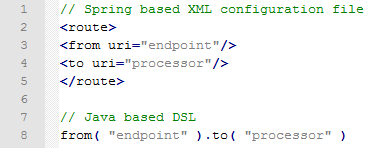
\includegraphics[scale=0.95]{camel.png} 
	\caption{Sposób definiowania ścieżek w technologii Apache Camel}
\end{figure}

W platformie SpeechProcessingPlatform technologia Apache Camel używana jest do komunikacji między poszczególnymi komponentami. Technologia ta dostarcza adresację oraz prosty interfejs do MOM.
	
\section{Technologie przetwarzania mowy}		
\subsection{FreeTTS}
FreeTTS \cite{freettssite} jest syntezatorem mowy, dostępnym na licencji opensource, w całości napisanym w języku Java. Bazuje na silniku Flite stworzonym i rozwijanym przez Carnegie Mellon University. Mimo swojej prostoty jego zaletami są duża wydajność, bardzo dobre radzenie sobie z językiem angielskim oraz częściowe wsparcie dla JSAPI 1.0(jako, że jest to syntezator nie wspiera częsci specyfikacji odpowiedzialnej za rozpoznawanie mowy). Dzięki temu ostatniemu w łatwy sposób umożliwia integrację z różnymi, wieloplatformowymi aplikacjami działającymi wewnątrz JVM. Przy opisywaniu tego syntezatora istotną kwestią jest fakt, że posiada dość dobrą dokumentację oraz liczne, łatwe do uruchomienia i, co bardzo ważne, działające dema. Standardowo oferuje 3 różne głosy, wszystkie w języku angielskim, umożliwia jednak rozszerzenie liczby głosów poprzez import nowych stworzonych przy pomocy narzędzi takich jak:
\begin{itemize}
	\item FestVox,
	\item MBROLA,
	\item CMU Arctic.
\end{itemize}    

\subsection{Ivona TTS}
IVONA TTS \cite{ivonasite} to wielojęzyczny syntetyzator mowy działający w oparciu o metodę alofoniczną. Autorski algorytm stosowany przez Ivona nazywa się Bright Voices,  powstał i został opisany podczas Blizzard Challenge 2006. W chwili obecnej funkcjonalność Ivona jest dostępna na dwa sposoby:
\begin{itemize}
	\item poprzez Ivona SDK
	\item poprzez Speech Cloud (SaaS)
\end{itemize}
Ivona SDK to podstawowy sposób korzystania z usług tego oprogramowania. Dostępne są wersję na wiele różnych platform takich jak:
\begin{itemize}
	\item Linux
	\item Windows
	\item iOS
	\item Solaris
\end{itemize}
oraz w kilku różnych językach programowania:
\begin{itemize}
	\item C/C++
	\item Java
	\item ObjectiveC
	\item platforma .NET
\end{itemize}
Dostęp do technologii Speech Cloud możliwy jest zarówno za pomocą protokołu SOAP oraz przez reprezentację technologii REST. W tej chwili niezależnie od używanego API można uzyskać następującą funkcjonalność:
\begin{itemize}
	\item wygenerowanie pliku dźwiękowego z podanego tekstu
	\item pobranie informacji o dostępnych głosach i kodekach
	\item zmodyfikowanie zasad wymowy, w celu poprawienia jakości wymowy niektórych słów
\end{itemize}
Syntezator ten wspiera bardzo dużo języków między innymi:
 \begin{itemize}
	\item polski
	\item angielski
	\item francuski
	\item portugalski
	\item niemiecki
\end{itemize}
Poza wyborem języka istnieje też możliwość wyboru lektora, różnią się oni barwą i siłą głosu, czy też szybkością mówienia. Możliwa jest też dynamiczna zmiana zarówno języka jak i lektora. Kolejną ważną cechą Ivona jest fakt, iż nie ogranicza się ona do jednego kodeka, wspiera następujące formaty:
\begin{itemize}
	\item mp3/22050
	\item ogg/22050
	\item pcm16/22050
	\item alaw/8000
\end{itemize}
 Aby korzystać ze zdalnego API należy posiadać konto w systemie Ivony, jest ono wykorzystywane do pobierania opłat. Co bardzo istotne, Ivona wspiera protokół SSML, umożliwiający klientowi dokładniejsze sterowanie generowanym głosem. 

\subsection{Google Translate}
Google Translate to płatna usługa Google umożliwiająca tłumaczenie tekstu pomiędzy tysiącami dostępnych par języków. Poza tłumaczeniem usługa ta umożliwia również rozpoznanie języka. API udostępniane przez korporację opiera się o architekturę REST, składa się z trzech metod:
\begin{itemize}
	\item translate - tłumaczy tekst z języka źródłowego na docelowy, przykład:
	\lstset{caption={Tłumaczenie słowa hello z angielskiego na polski},label=DescriptiveLabel}
	\begin{lstlisting}
	https://www.googleapis.com/language/translate/v2?key=INSERT-YOUR-KEY&q=hello%20world&source=en&target=pl
	\end{lstlisting}
	\item languages - zwraca listę języków wspieranych przez translator
	\lstset{caption={Przykład pobrania listy dostępnych języków},label=DescriptiveLabel}
	\begin{lstlisting}
	https://www.googleapis.com/language/translate/v2/languages?key=INSERT-YOUR-KEY&target=zh-TW
	\end{lstlisting}
	\item detect - rozpoznaje język tekstu źródłowego
	\lstset{caption={Przykład detekcji języka},label=DescriptiveLabel}
	\begin{lstlisting}
	https://www.googleapis.com/language/translate/v2/detect?key=INSERT-YOUR-KEY&q=google+translate+is+fast
	\end{lstlisting}
\end{itemize}
Parametr key=INSERT-YOUR-KEY służy korporacji do identyfikowania usługobiorcy, na jego podstawie naliczane są opłaty. Jak widać REST w API Google Translate różni się nieznacznie od tradycyjnego pojmowania tej architektury. Zamiast dostarczać dostęp do zasobów, dostarczany jest dostęp do usług, stosując takie podejście uzyskano możliwość wykorzystania jednego URI jako całego API. 

\subsection{OCR Web Service}
OCR Web Service jest to jeden z najpopularniejszych technologii web serwices tego rodzaju. Rozpoznaje aż dwadzieścia osiem języków między innymi:
\begin{itemize}
	\item polski
	\item angielski
	\item niemiecki
	\item francuski
	\item portugalski
\end{itemize}
Przyjmuje różne formaty wejściowe, takie jak: JPEG/JPG, BMP, PCX, GIF, PNG, PDF. Co więcej pozwala na przekonwertowanie rozpoznanego tekstu na aż sześć różnych formatów:
\begin{itemize}
	\item Adobe PDF
	\item MS Word 2003
	\item MS Excel 2003
	\item HTML
	\item RTF
\end{itemize}
Oczywiście istnieje też możliwość otrzymania zwykłego pliku txt. Wymagania tej usługi co do jakości obrazu w pliku otrzymanym na wejściu też nie są duże, zaleca się aby rozdzielczość wynosiła między 200 a 400 dpi. Usługa ta, jako protokół komunikacyjny wykorzystuje SOAP w wersji 1.1 lub 1.2. WSDL potrzebny do wygenerowania szkieletu kodu można pobrać ze strony projektu. Jedną z niewielu wad tej usługi jest to, że podobnie jak Google Translate jest płatna. 